% !TEX program = xelatex
\documentclass[10pt,letterpaper,twocolumn]{article}

% === GEOMETRY ===
\usepackage[top=0.75in, bottom=0.75in, left=0.75in, right=0.75in]{geometry}

% === FONTS ===
\usepackage{fontspec}
\usepackage{unicode-math}

\setmainfont{Latin Modern Roman}
\setsansfont{Latin Modern Sans}

% Custom AC fonts
\newfontfamily\acbold{ywft-processing-bold}[
  Path=../../system/public/type/webfonts/,
  Extension=.ttf
]
\newfontfamily\aclight{ywft-processing-light}[
  Path=../../system/public/type/webfonts/,
  Extension=.ttf
]
\newfontfamily\kidlispfont{ComicRelief-Regular}[
  Path=../arxiv-kidlisp/fonts/,
  Extension=.ttf
]
\newfontfamily\kidlispbold{ComicRelief-Bold}[
  Path=../arxiv-kidlisp/fonts/,
  Extension=.ttf
]
\setmonofont{Latin Modern Mono}[Scale=0.85]

% === PACKAGES ===
\usepackage{xcolor}
\usepackage{titlesec}
\usepackage{enumitem}
\usepackage{booktabs}
\usepackage{tabularx}
\usepackage{fancyhdr}
\usepackage{hyperref}
\usepackage{graphicx}
\graphicspath{{figures/}{../arxiv-kidlisp/figures/}}
\usepackage{ragged2e}
\usepackage{microtype}
\usepackage{listings}
\usepackage{natbib}
\usepackage[colorspec=0.92]{draftwatermark}

% === COLORS (AC palette) ===
\definecolor{acpink}{RGB}{180,72,135}
\definecolor{acpurple}{RGB}{120,80,180}
\definecolor{acdark}{RGB}{64,56,74}
\definecolor{acgray}{RGB}{119,119,119}
\definecolor{klbrand}{RGB}{205,92,155}
\definecolor{klcyan}{RGB}{112,214,255}
\definecolor{kldark}{RGB}{48,43,58}
\definecolor{draftcolor}{RGB}{205,92,155}

% === DRAFT WATERMARK ===
\DraftwatermarkOptions{
  text=BORRADOR,
  fontsize=3cm,
  color=draftcolor!18,
  angle=45,
  pos={0.5\paperwidth, 0.5\paperheight}
}

% === KIDLISP SYNTAX COLORS ===
\definecolor{klfn}{RGB}{0,136,170}
\definecolor{klform}{RGB}{119,51,170}
\definecolor{klrepeat}{RGB}{170,0,170}
\definecolor{klnum}{RGB}{204,0,102}
\definecolor{klstr}{RGB}{170,120,0}
\definecolor{klcmt}{RGB}{102,102,102}
\definecolor{klmath}{RGB}{0,136,0}
\definecolor{klvar}{RGB}{204,102,0}
\definecolor{klembed}{RGB}{0,136,0}

% KidLisp inline color macros
\newcommand{\kn}[1]{\textcolor{klnum}{#1}}
\newcommand{\kt}[1]{\textcolor{klstr}{#1}}
\newcommand{\kv}[1]{\textcolor{klvar}{#1}}
\newcommand{\ke}[1]{\textcolor{klembed}{\textbf{#1}}}
\newcommand{\km}[1]{\textcolor{klmath}{#1}}

% === HYPERREF ===
\hypersetup{
  colorlinks=true,
  linkcolor=acpurple,
  urlcolor=acpurple,
  citecolor=acpurple,
  pdfauthor={@jeffrey},
  pdftitle={Tarjetas KidLisp: Programas que caben en una tarjeta},
}

% === SECTION FORMATTING ===
\titleformat{\section}
  {\normalfont\bfseries\normalsize\uppercase}
  {\thesection.}
  {0.5em}
  {}
\titlespacing{\section}{0pt}{1.2em}{0.3em}

\titleformat{\subsection}
  {\normalfont\bfseries\small}
  {\thesubsection}
  {0.5em}
  {}
\titlespacing{\subsection}{0pt}{0.8em}{0.2em}

% === HEADER/FOOTER ===
\pagestyle{fancy}
\fancyhf{}
\renewcommand{\headrulewidth}{0pt}
\fancyhead[C]{\footnotesize\color{acpink}\textit{Borrador de trabajo --- no citar}}
\fancyfoot[C]{\footnotesize\thepage}

% === CUSTOM COMMANDS ===
\newcommand{\acdot}{{\color{acpink}.}}
\newcommand{\kidlisp}{\textsc{KidLisp}}

% === LISTINGS ===
\lstdefinelanguage{kidlisp}{
  morekeywords=[1]{wipe,ink,line,box,circle,tri,plot,flood,shape,zoom,scroll,spin,blur,contrast,embed,layer,width,height,frame,time,wiggle,melody,mic,suck,sort,form,trans,cube,move,scale,hop,overtone,resolution,write,text,type,stamp,paste,point,poly,noise,fade,pan,unpan,mask,unmask,flip,crawl,left,right,up,down,goto,face,outline,fill,stroke},
  morekeywords=[2]{def,let,if,cond,once,later,lambda,do},
  morekeywords=[3]{repeat},
  morekeywords=[4]{random,sin,cos,tan,floor,ceil,round,abs,sqrt,min,max},
  sensitive=true,
  morecomment=[l]{;},
  morestring=[b]",
  escapeinside={|}{|},
}
\lstset{
  language=kidlisp,
  basicstyle=\ttfamily\small,
  keywordstyle=[1]\color{klfn}\bfseries,
  keywordstyle=[2]\color{klform}\bfseries,
  keywordstyle=[3]\color{klrepeat}\bfseries,
  keywordstyle=[4]\color{klmath},
  commentstyle=\color{klcmt}\itshape,
  stringstyle=\color{klstr},
  breaklines=true,
  frame=single,
  rulecolor=\color{acgray!30},
  backgroundcolor=\color{acgray!5},
  xleftmargin=0.5em,
  xrightmargin=0.5em,
  aboveskip=0.5em,
  belowskip=0.5em,
}

\lstdefinelanguage{python}{
  morekeywords={def,return,import,from,class,if,else,for,in,with,as,try,except,None,True,False,self,and,or,not,lambda,yield,pass,break,continue,raise,while},
  sensitive=true,
  morecomment=[l]{\#},
  morestring=[b]",
  morestring=[b]',
}
\lstset{
  language=kidlisp,
}

% === LIST SETTINGS ===
\setlist[itemize]{nosep, leftmargin=1.2em, itemsep=0.1em}
\setlist[enumerate]{nosep, leftmargin=1.2em}

% === COLUMN SEPARATION ===
\setlength{\columnsep}{1.8em}

% === PARAGRAPH SETTINGS ===
\setlength{\parindent}{1em}
\setlength{\parskip}{0.3em}

\tolerance=800
\emergencystretch=1em
\hyphenpenalty=50

\begin{document}

% ============ TITLE BLOCK ============

\twocolumn[{%
\begin{center}

\includegraphics[height=4em]{pals}\par\vspace{0.5em}
{\kidlispbold\fontsize{24pt}{28pt}\selectfont\color{kldark} Kid{\color{klbrand}Lisp} Tarjetas}\par
\vspace{0.2em}
{\kidlispfont\fontsize{11pt}{13pt}\selectfont\color{klbrand} Programas que caben en una tarjeta}\par
\vspace{0.6em}
{\normalsize\href{https://prompt.ac/@jeffrey}{@jeffrey}}\par
{\small\color{acgray} Aesthetic\acdot Computer}\par
{\small\color{acgray} ORCID: \href{https://orcid.org/0009-0007-4460-4913}{0009-0007-4460-4913}}\par
\vspace{0.3em}
{\small\color{acpurple} \url{https://kidlisp.com} \enspace$\cdot$\enspace \url{https://aesthetic.computer}}\par
\vspace{0.6em}
\rule{\textwidth}{1.5pt}
\vspace{0.5em}
\end{center}

\begin{center}
{\small\color{acpink}\textbf{[ borrador de trabajo --- no citar ]}}
\end{center}
\vspace{0.3em}

\begin{quote}
\small\noindent\textbf{Resumen.}
Los programas de \kidlisp{} son cortos. Un programa t\'ipico consta de 2--4 l\'ineas de S-expresiones que producen una composici\'on visual completa---una explosi\'on estelar, una espiral, un mosaico, un fractal. Esta brevedad no es incidental sino dise\~nada: el lenguaje omite funciones definidas por el usuario, recursi\'on y mecanismos de abstracci\'on, de modo que los programas permanecen planos y legibles. Observamos que esta planitud crea una correspondencia natural entre programas y tarjetas f\'isicas. Un programa de \kidlisp{}, su c\'odigo fuente y su salida renderizada pueden coexistir en una sola tarjeta impresa. Este art\'iculo describe el formato \emph{KidLisp Cards}---una baraja de programas organizados por categor\'ia visual---y un pipeline de renderizado en Python (int\'erprete basado en PIL) que produce im\'agenes de tarjetas fuera del navegador. Discutimos qu\'e son las tarjetas ahora (un cuaderno curado de koans visuales), en qu\'e podr\'ian convertirse (tarjetas coleccionables, secuencias pedag\'ogicas, partituras impresas, arte postal), y c\'omo la restricci\'on de la tarjeta retroalimenta el dise\~no del lenguaje.
\end{quote}
\vspace{0.5em}
}]

% ============ 1. INTRODUCCI\'ON ============

\section{Introducci\'on}

La mayor\'ia de los lenguajes de programaci\'on producen programas demasiado largos para imprimir en una ficha. Esto es consecuencia de la abstracci\'on: los lenguajes de prop\'osito general fomentan la descomposici\'on en funciones, clases, m\'odulos y archivos. El programa se distribuye a trav\'es de una base de c\'odigo. Ning\'un artefacto individual captura el todo.

\kidlisp{} es diferente. Sus programas tienen t\'ipicamente 1--6 l\'ineas de largo. Una escena animada completa, un patr\'on geom\'etrico, un fractal recursivo o un patr\'on de interferencia moir\'{e} cabe en unas pocas S-expresiones. Esto no es una limitaci\'on sino una elecci\'on de dise\~no: \kidlisp{} omite funciones definidas por el usuario, recursi\'on (excepto a trav\'es de \texttt{later}), estructuras de datos mutables e importaciones. Los programas son secuencias planas de comandos de dibujo, bucles y condicionales.

Esta planitud crea una oportunidad. Si el c\'odigo fuente de un programa cabe en una tarjeta, y la salida visual de ese programa cabe en la misma tarjeta, entonces la tarjeta se convierte en un artefacto autocontenido: un programa que puedes sostener, pasar a alguien, clavar en una pared o enviar por correo. La tarjeta es tanto documentaci\'on como ejecutable. Es una \emph{partitura}---instrucciones para producir un evento visual.

Este art\'iculo describe el formato KidLisp Cards (\S\ref{sec:format}), el pipeline de renderizado offline (\S\ref{sec:pipeline}), el cat\'alogo actual de tarjetas (\S\ref{sec:catalog}), las variaciones de disposici\'on y sus affordances sociales y f\'isicas (\S\ref{sec:layouts}), y futuros especulativos para el formato (\S\ref{sec:futures}).

% ============ 2. EL FORMATO DE TARJETA ============

\section{El formato de tarjeta}
\label{sec:format}

Una tarjeta KidLisp tiene tres elementos:

\begin{enumerate}
  \item \textbf{T\'itulo.} Un nombre corto que evoca la salida visual: ``Starburst,'' ``Honeycomb,'' ``Spiral Walk.''
  \item \textbf{Salida renderizada.} Una imagen de pixel art (resoluci\'on predeterminada de 160$\times$120, escalada 3$\times$ con interpolaci\'on de vecino m\'as cercano para preservar bordes n\'itidos).
  \item \textbf{C\'odigo fuente.} El programa \kidlisp{} completo, t\'ipicamente 1--4 l\'ineas, mostrado en monoespaciado debajo de la imagen.
\end{enumerate}

La tarjeta es autocontenida: cualquiera que lea el c\'odigo fuente puede reproducir la imagen exactamente, en cualquier int\'erprete de \kidlisp{}. No hay dependencias externas, no hay importaciones, no hay configuraci\'on. El programa \emph{es} la tarjeta.

\subsection{Dimensiones de la tarjeta}

La imagen renderizada ocupa un lienzo de 160$\times$120 p\'ixeles (proporci\'on 4:3), coincidiendo con la resoluci\'on predeterminada de \kidlisp{}. A 3$\times$ de escala, esto produce una imagen de 480$\times$360 p\'ixeles adecuada para visualizaci\'on en pantalla. Para impresi\'on, las tarjetas miden 4$\times$6 pulgadas (ficha est\'andar / postal), con la imagen en la parte superior y el c\'odigo fuente debajo.

\subsection{Qu\'e hace una buena tarjeta}

No todo programa de \kidlisp{} produce una buena tarjeta. Las mejores tarjetas comparten propiedades:

\begin{itemize}
  \item \textbf{Brevedad.} 1--4 l\'ineas. Si el c\'odigo fuente no cabe c\'omodamente debajo de la imagen, el programa es demasiado largo para el formato.
  \item \textbf{Sorpresa.} La salida debe ser m\'as compleja o bella de lo que sugiere el c\'odigo fuente. Un programa de tres l\'ineas que produce un patr\'on moir\'{e} recompensa la inspecci\'on.
  \item \textbf{Legibilidad.} Un lector deber\'ia poder trazar desde la fuente hasta la salida sin ejecutar el programa. La conexi\'on entre c\'odigo e imagen debe ser discernible, aunque no sea inmediatamente obvia.
  \item \textbf{Independencia.} Sin incrustaciones \texttt{\$code}, sin estado externo. La tarjeta debe funcionar de forma aislada.
\end{itemize}

\begin{figure}[t]
\centering
\fbox{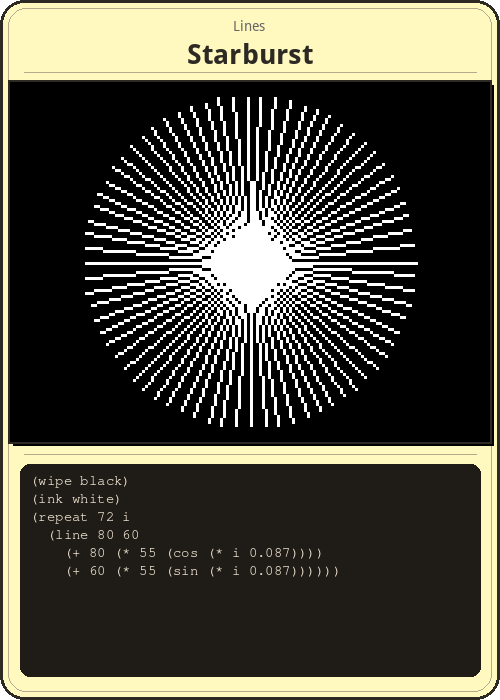
\includegraphics[width=0.47\columnwidth]{card-starburst.png}}%
\hfill%
\fbox{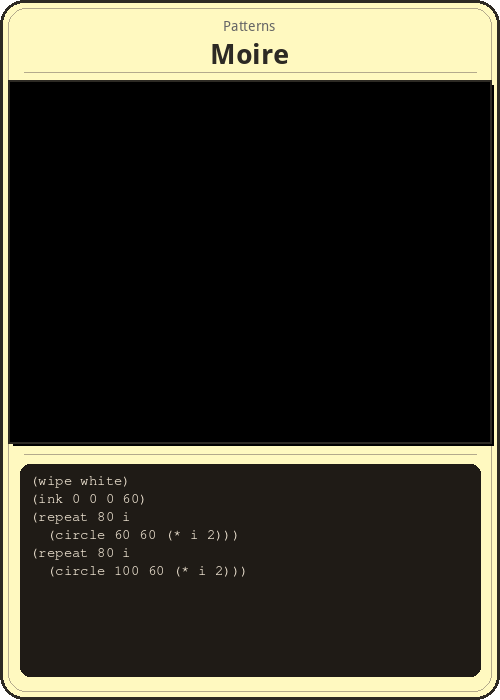
\includegraphics[width=0.47\columnwidth]{card-moire.png}}
\caption{Dos tarjetas de programa renderizadas por el int\'erprete Python: ``Starburst'' (72 l\'ineas radiales, 3 l\'ineas de c\'odigo) y ``Moir\'{e}'' (c\'irculos conc\'entricos superpuestos, 3 l\'ineas). Estos son ejemplos triviales---demuestran la estructura del formato de tarjeta pero no representan el rango expresivo del lenguaje ni las ambiciones del formato.}
\label{fig:program-cards}
\end{figure}

% ============ 3. PIPELINE DE RENDERIZADO ============

\section{Pipeline de renderizado offline}
\label{sec:pipeline}

Las tarjetas KidLisp se renderizan usando un int\'erprete Python que se ejecuta fuera del navegador. Esto permite el renderizado por lotes, la producci\'on para impresi\'on y la curaci\'on basada en cuadernos sin requerir el runtime completo de Aesthetic\acdot Computer.

\subsection{El int\'erprete Python}

El int\'erprete (\texttt{notebooks/ac.py}, 452 l\'ineas) implementa un subconjunto de \kidlisp{} suficiente para el renderizado est\'atico de tarjetas:

\begin{itemize}
  \item \textbf{Dibujo:} \texttt{wipe}, \texttt{ink}, \texttt{line}, \texttt{box}, \texttt{circle}, \texttt{tri}, \texttt{plot}, \texttt{shape}, \texttt{flood}
  \item \textbf{Tortuga:} \texttt{crawl}, \texttt{left}, \texttt{right}, \texttt{goto}, \texttt{face}, \texttt{up}, \texttt{down}
  \item \textbf{Control:} \texttt{repeat}, \texttt{if}, \texttt{def}, \texttt{later}, \texttt{do}
  \item \textbf{Matem\'aticas:} aritm\'etica completa, trigonometr\'ia, \texttt{abs}, \texttt{sqrt}, \texttt{min}, \texttt{max}
  \item \textbf{Lienzo:} \texttt{resolution}, \texttt{fill}, \texttt{outline}, \texttt{stroke}
\end{itemize}

El int\'erprete usa PIL (Pillow) para el renderizado. Cada tarjeta se dibuja en un lienzo RGBA, se escala con interpolaci\'on de vecino m\'as cercano y se exporta como PNG. La implementaci\'on en Python es intencionalmente m\'as simple que el evaluador del navegador (15.161 l\'ineas)---omite animaci\'on, audio, incrustaci\'on y sintaxis de temporizaci\'on, centr\'andose solo en el subconjunto necesario para la salida visual est\'atica.

\subsection{Flujo de trabajo con Jupyter Notebook}

La herramienta principal de curaci\'on es un cuaderno Jupyter (\texttt{notebooks/kidlisp-cards.ipynb}). La funci\'on \texttt{show\_card()} renderiza un programa y lo muestra en l\'inea como una tarjeta HTML:

\begin{lstlisting}[language=python,basicstyle=\ttfamily\footnotesize]
show_card("Starburst", """(wipe black)
(ink white)
(repeat 72 i
  (line 80 60
    (+ 80 (* 55 (cos (* i 0.087))))
    (+ 60 (* 55 (sin (* i 0.087))))))""")
\end{lstlisting}

Cada llamada produce una tarjeta con fondo oscuro con el t\'itulo, la imagen renderizada y el c\'odigo fuente mostrados en l\'inea. El cuaderno sirve tanto como entorno de desarrollo como galer\'ia---desplazarse por el cuaderno es como hojear una baraja de tarjetas.

\subsection{Dos int\'erpretes, un lenguaje}

La existencia de dos int\'erpretes independientes (JavaScript en el navegador, Python en el cuaderno) sirve como mecanismo de validaci\'on cruzada. Si un programa se renderiza de forma id\'entica en ambos, su comportamiento est\'a determinado enteramente por la sem\'antica del lenguaje y no por detalles de implementaci\'on. Los programas que dependen de caracter\'isticas espec\'ificas del navegador (animaci\'on, audio, capas incrustadas) quedan excluidos del formato de tarjeta por construcci\'on---simplemente no se renderizan en el int\'erprete Python.

% ============ 4. CAT\'ALOGO DE TARJETAS ============

\section{El cat\'alogo de tarjetas}
\label{sec:catalog}

El cuaderno actual contiene 28 tarjetas organizadas en siete categor\'ias. Cada categor\'ia explora un aspecto diferente del lenguaje a trav\'es de ejemplos m\'inimos. Estos programas son deliberadamente triviales---ejercicios de dibujo, ilustraciones matem\'aticas, caminatas de tortuga. Establecen la estructura del formato de tarjeta pero no representan su potencial expresivo. Las tarjetas interesantes a\'un no se han hecho. El valor del formato surgir\'a de programas que usen la brevedad para decir algo que valga la pena decir, no de demos geom\'etricas.

\subsection{L\'ineas}

Las tarjetas de l\'ineas demuestran \texttt{repeat} y trigonometr\'ia. Una explosi\'on estelar irradia 72 l\'ineas desde el centro. Un entrecruzado superpone rejillas horizontales y verticales con baja opacidad.

\begin{figure}[h]
\centering
\fbox{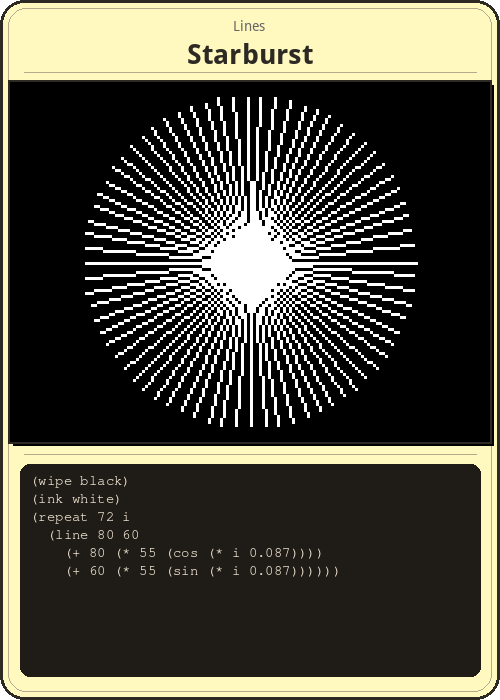
\includegraphics[width=0.47\columnwidth]{card-starburst.png}}%
\hfill%
\fbox{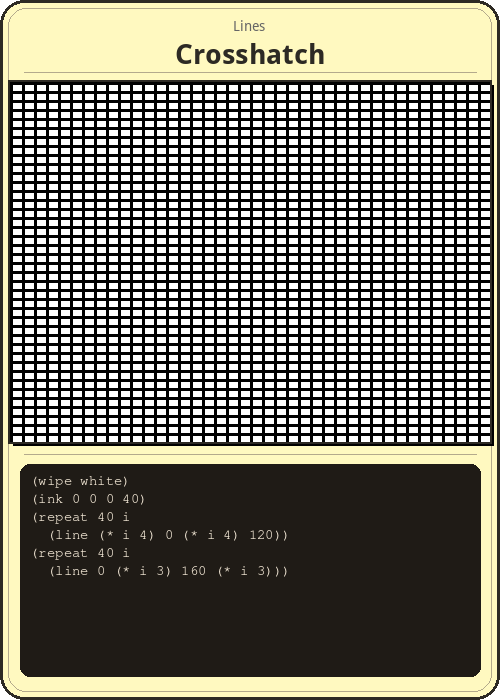
\includegraphics[width=0.47\columnwidth]{card-crosshatch.png}}
\caption{``Starburst'' y ``Crosshatch'' --- tarjetas de l\'ineas.}
\label{fig:lines}
\end{figure}

\begin{lstlisting}
; Starburst — 72 radial lines
(wipe |\kt{black}|)
(ink |\kt{white}|)
(repeat |\kn{72}| |\kv{i}|
  (line |\kn{80}| |\kn{60}|
    (|\km{+}| |\kn{80}| (|\km{*}| |\kn{55}| (|\km{cos}| (|\km{*}| |\kv{i}| |\kn{0.087}|))))
    (|\km{+}| |\kn{60}| (|\km{*}| |\kn{55}| (|\km{sin}| (|\km{*}| |\kv{i}| |\kn{0.087}|))))))
\end{lstlisting}

\subsection{C\'irculos}

Las tarjetas de c\'irculos usan el modo \texttt{outline} y bucles \texttt{repeat} anidados. ``Ripple'' dibuja 30 c\'irculos conc\'entricos con color que cambia hacia el azul.

\begin{figure}[h]
\centering
\fbox{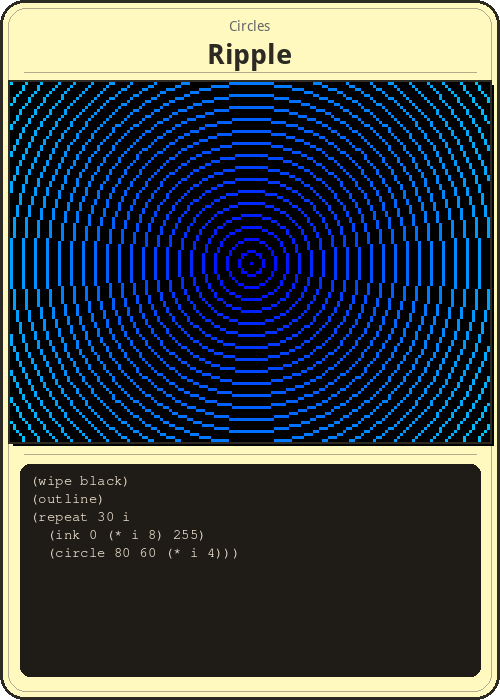
\includegraphics[width=0.47\columnwidth]{card-ripple.png}}%
\hfill%
\fbox{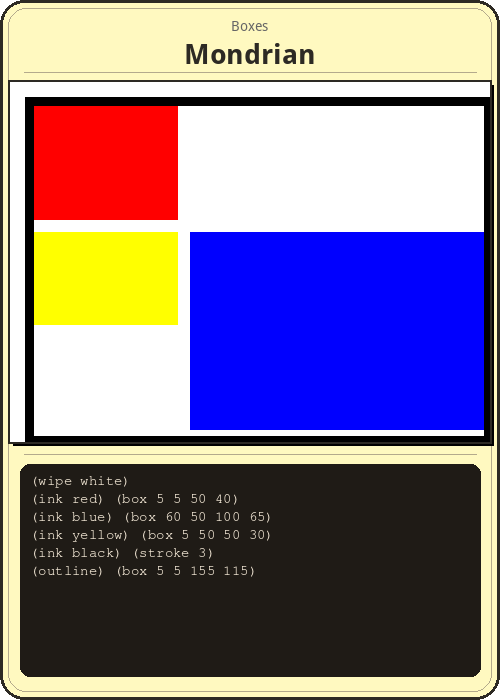
\includegraphics[width=0.47\columnwidth]{card-mondrian.png}}
\caption{``Ripple'' (c\'irculos) y ``Mondrian'' (cajas).}
\label{fig:circles-boxes}
\end{figure}

\subsection{Cajas y composici\'on}

``Mondrian'' recrea la rejilla de colores primarios con cuatro rect\'angulos coloreados. ``Nest'' dibuja 10 rect\'angulos insertados con tonos cambiantes.

\subsection{Matem\'aticas y curvas}

Estas tarjetas usan \texttt{plot} con funciones matem\'aticas. ``Lissajous'' dibuja una figura de Lissajous con 600 puntos. ``Spiral'' traza una espiral polar.

\begin{figure}[h]
\centering
\fbox{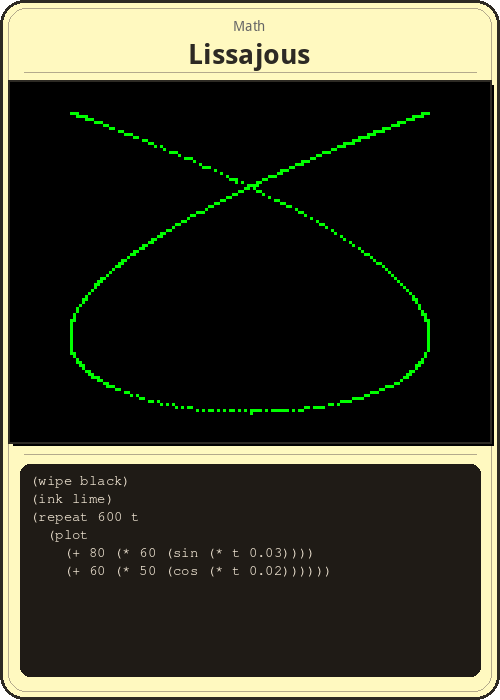
\includegraphics[width=0.47\columnwidth]{card-lissajous.png}}%
\hfill%
\fbox{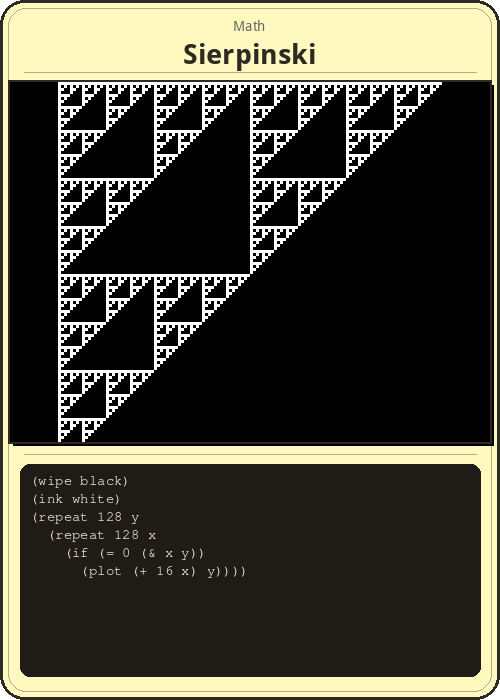
\includegraphics[width=0.47\columnwidth]{card-sierpinski.png}}
\caption{``Lissajous'' (curvas matem\'aticas) y ``Sierpinski'' (fractal AND a nivel de bits).}
\label{fig:math}
\end{figure}

\subsection{Color y gradientes}

``Sierpinski'' usa AND a nivel de bits para generar el tri\'angulo de Sierpinski: \texttt{(if (= 0 (\& x y)) (plot (+ 16 x) y))}. ``Sunflower'' traza 500 puntos a lo largo de una espiral de \'angulo \'aureo con colores c\'iclicos.

\subsection{Gr\'aficos de tortuga}

Las tarjetas de tortuga usan \texttt{crawl}, \texttt{left}, \texttt{right} y \texttt{face}. Una estrella de cinco puntas usa \texttt{(right 144)}. Un \'arbol usa \texttt{later} para ramificaci\'on recursiva. Un copo de nieve anida segmentos de curva de Koch.

\begin{figure}[h]
\centering
\fbox{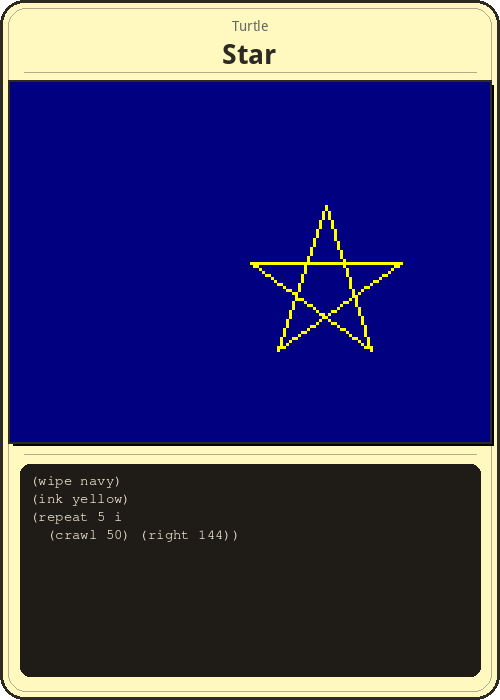
\includegraphics[width=0.47\columnwidth]{card-star.png}}%
\hfill%
\fbox{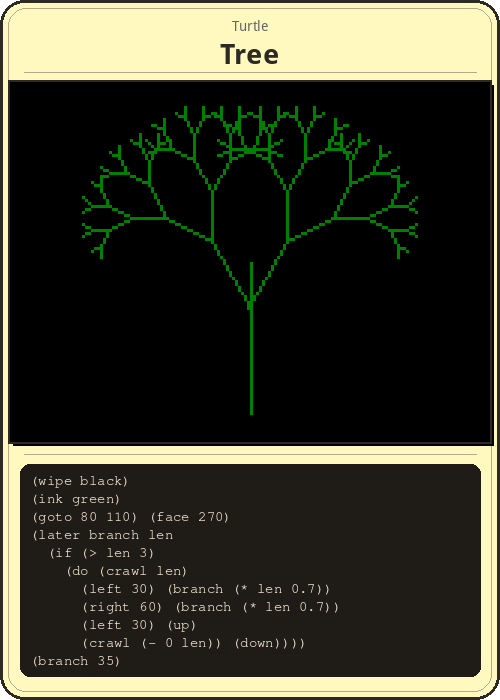
\includegraphics[width=0.47\columnwidth]{card-tree.png}}
\caption{``Star'' y ``Tree'' --- tarjetas de gr\'aficos de tortuga.}
\label{fig:turtle}
\end{figure}

\begin{lstlisting}
; Star — 5 sides, 144-degree turns
(wipe |\kt{navy}|)
(ink |\kt{yellow}|)
(repeat |\kn{5}| |\kv{i}| (crawl |\kn{50}|) (right |\kn{144}|))
\end{lstlisting}

\subsection{Koans m\'inimos}

Las tarjetas m\'as cortas de la baraja. ``Horizon'' son tres l\'ineas: cielo oscuro, tierra dorada. ``Pip'' es un solo punto rojo sobre negro. Estas tarjetas se acercan al programa m\'inimo viable---la menor cantidad de c\'odigo que produce una imagen reconocible.

\begin{figure}[h]
\centering
\fbox{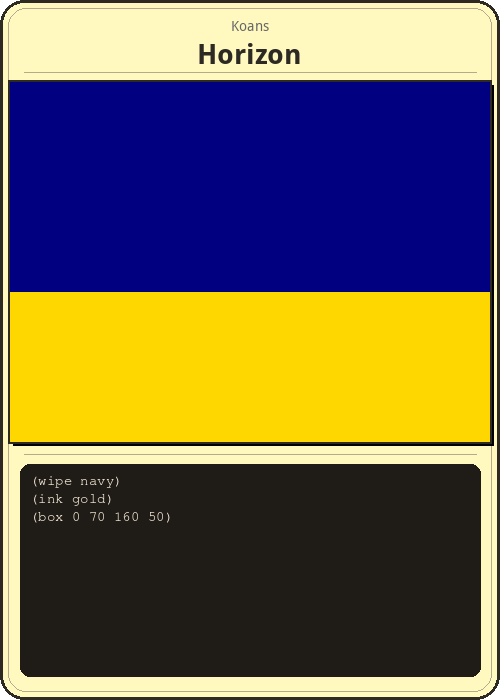
\includegraphics[width=0.47\columnwidth]{card-horizon.png}}%
\hfill%
\fbox{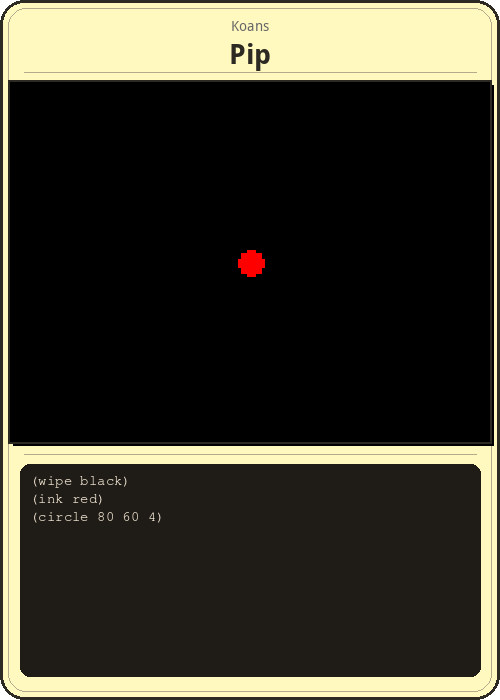
\includegraphics[width=0.47\columnwidth]{card-pip.png}}
\caption{``Horizon'' y ``Pip'' --- koans m\'inimos (2--3 l\'ineas cada uno).}
\label{fig:koans}
\end{figure}

\begin{lstlisting}
; Pip — the minimum card
(wipe |\kt{black}|)
(ink |\kt{red}|)
(circle |\kn{80}| |\kn{60}| |\kn{4}|)
\end{lstlisting}

\begin{figure*}[t]
\centering
\fbox{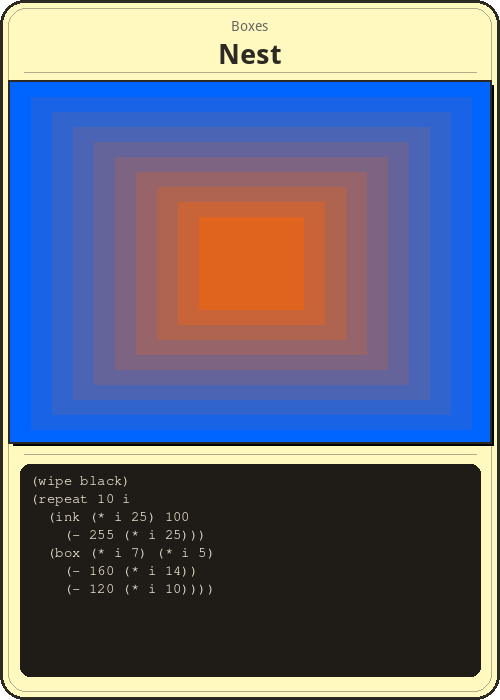
\includegraphics[height=5.5cm]{card-nest.png}}%
\hfill%
\fbox{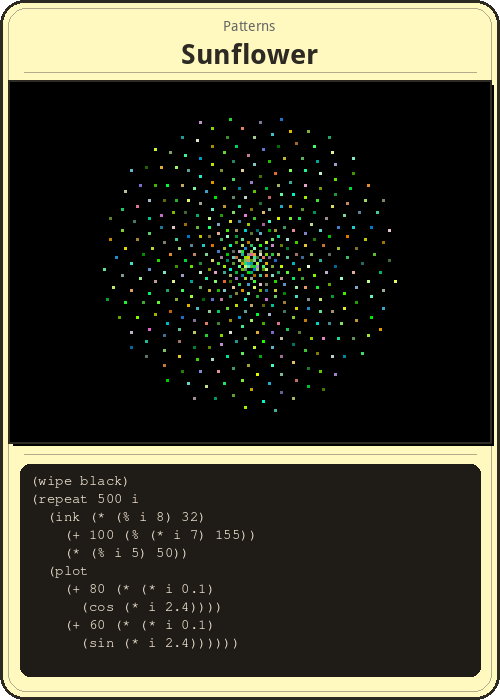
\includegraphics[height=5.5cm]{card-sunflower.png}}%
\hfill%
\fbox{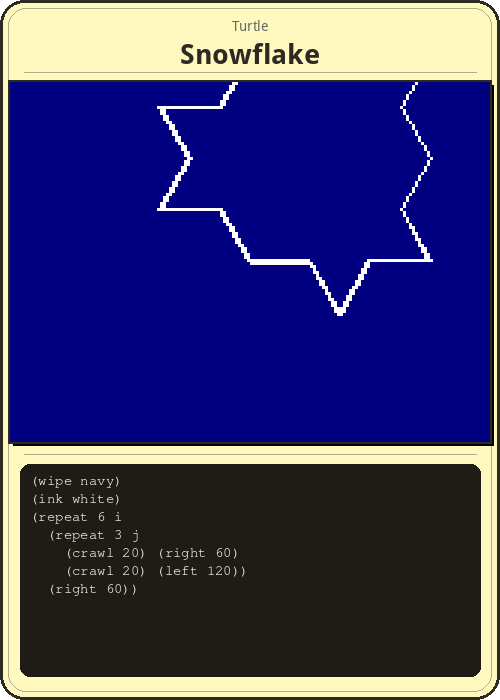
\includegraphics[height=5.5cm]{card-snowflake.png}}%
\hfill%
\fbox{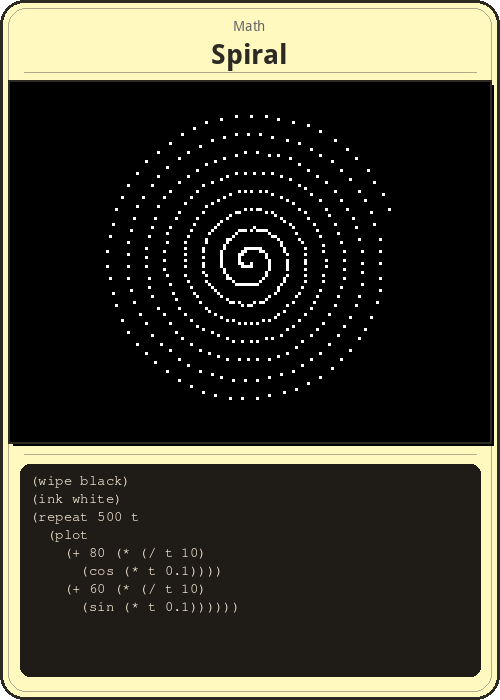
\includegraphics[height=5.5cm]{card-spiral.png}}
\caption{Cuatro tarjetas completas que muestran el formato: t\'itulo, salida renderizada y c\'odigo fuente. De izquierda a derecha: ``Nest,'' ``Sunflower,'' ``Snowflake,'' ``Spiral.'' Cada tarjeta es autocontenida---el c\'odigo fuente debajo de la imagen es el programa completo. Estos son ejercicios de dibujo triviales, no expresiones del potencial del formato.}
\label{fig:four-cards}
\end{figure*}

% ============ 5. DISPOSICIONES ============

\section{Disposiciones}
\label{sec:layouts}

El formato de tarjeta no tiene una disposici\'on fija. C\'omo se organizan los tres elementos (t\'itulo, salida, fuente) determina lo que la tarjeta permite---lo que puedes hacer con ella f\'isica y socialmente. Esta secci\'on explora variaciones de disposici\'on y sus consecuencias.

\begin{figure*}[t]
\centering
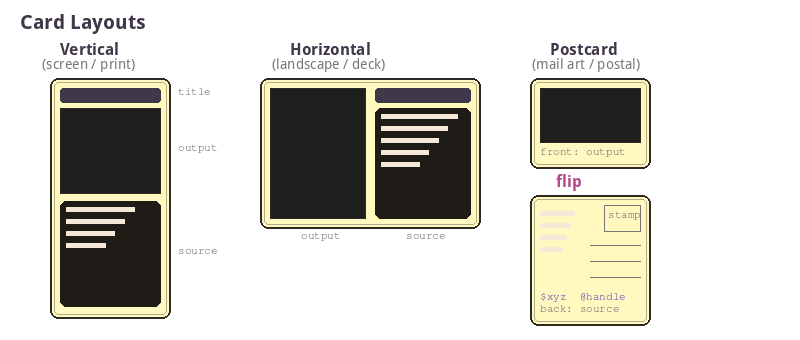
\includegraphics[width=\textwidth]{layout-comparison.png}
\caption{Tres estrategias de disposici\'on. \textbf{Vertical:} t\'itulo / imagen / fuente apilados de arriba a abajo, optimizado para pantallas de tel\'efono e impresi\'on en retrato. \textbf{Horizontal:} imagen a la izquierda, t\'itulo y fuente a la derecha, adecuado para tarjetas en paisaje y navegaci\'on de baraja lado a lado. \textbf{Postal:} salida renderizada en el frente, c\'odigo fuente y metadatos en el reverso---una tarjeta enviable por correo donde el programa est\'a oculto hasta que la volteas.}
\label{fig:layouts}
\end{figure*}

\subsection{Vertical (pantalla / impresi\'on)}

La disposici\'on predeterminada apila t\'itulo, imagen y fuente de arriba a abajo. Esta es la disposici\'on del cuaderno---se desplaza naturalmente en un tel\'efono o en un cuaderno Jupyter. Para impresi\'on, corresponde a una tarjeta de 4$\times$6 pulgadas en orientaci\'on retrato. El ojo del lector se mueve hacia abajo desde el nombre hasta la imagen y el c\'odigo, trazando la relaci\'on entre el programa y su salida.

\subsection{Horizontal (baraja / paisaje)}

Una disposici\'on en paisaje coloca la imagen renderizada a la izquierda y el c\'odigo fuente a la derecha. Esto funciona para desplegar tarjetas sobre una mesa, para presentaciones y para comparaci\'on lado a lado. Dos tarjetas colocadas una junto a otra crean un d\'iptico---el espectador puede comparar programas y salidas simult\'aneamente.

\subsection{Postal (arte postal)}

La disposici\'on postal separa el frente del reverso. El frente muestra solo la imagen renderizada, a sangre completa, sin texto. El reverso muestra el c\'odigo fuente, el handle del autor, el c\'odigo corto (\texttt{\$xyz}) y un \'area para sello. El destinatario ve la imagen primero---un artefacto visual. Voltear la tarjeta revela el programa: las instrucciones que lo produjeron. La tarjeta es tanto objeto art\'istico como partitura ejecutable, dependiendo de qu\'e lado leas.

\begin{figure*}[h]
\centering
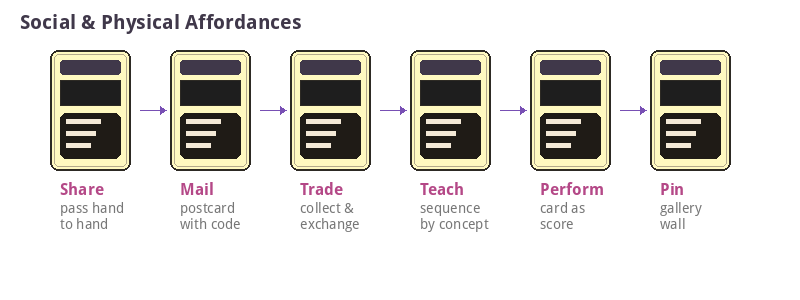
\includegraphics[width=\textwidth]{layout-affordances.png}
\caption{Affordances sociales y f\'isicas del formato de tarjeta. Cada affordance se deriva de la materialidad de la tarjeta: puede \textbf{compartirse} de mano en mano, \textbf{enviarse} como postal, \textbf{intercambiarse} y coleccionarse, \textbf{ense\~narse} en secuencias pedag\'ogicas, \textbf{interpretarse} como partitura gr\'afica o \textbf{colgarse} en la pared de una galer\'ia.}
\label{fig:affordances}
\end{figure*}

\subsection{Arreglos de baraja}

Las tarjetas no son objetos individuales. Forman barajas, y el arreglo de una baraja crea significado. Una \emph{secuencia pedag\'ogica} ordena tarjetas por concepto: cajas primero (coordenadas), luego l\'ineas (trigonometr\'ia), luego c\'irculos (radio y repetici\'on), luego curvas matem\'aticas (plot y seno), luego gr\'aficos de tortuga (movimiento relativo) y finalmente koans (expresi\'on m\'inima). Una \emph{cuadr\'icula de galer\'ia} arregla tarjetas espacialmente en una pared, invitando a la comparaci\'on entre categor\'ias. Una \emph{baraja mezclada} aleatoriza el orden, produciendo yuxtaposiciones inesperadas entre un fractal y un horizonte, entre un \'arbol y un punto.

\begin{figure}[h]
\centering
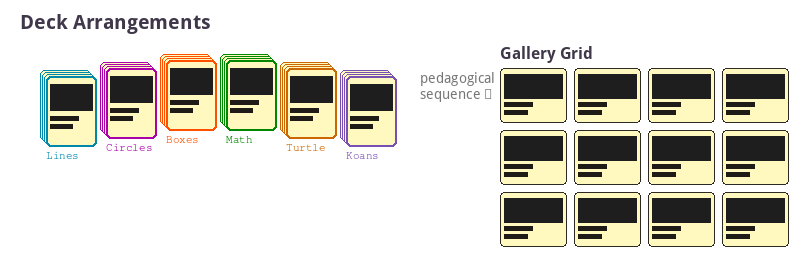
\includegraphics[width=\columnwidth]{layout-decks.png}
\caption{Arreglos de baraja. Izquierda: tarjetas desplegadas por categor\'ia (l\'ineas, c\'irculos, cajas, matem\'aticas, tortuga, koans) con m\'ultiples tarjetas apiladas por categor\'ia. Derecha: una cuadr\'icula de galer\'ia donde las tarjetas est\'an arregladas espacialmente para su navegaci\'on.}
\label{fig:decks}
\end{figure}

% ============ 6. TARJETAS EN EL MUNDO REAL ============

\section{Tarjetas en el mundo real}
\label{sec:wild}

Las tarjetas del cuaderno son ejercicios. El verdadero corpus de \kidlisp{}---m\'as de 16.000 programas creados por 59 autores---contiene piezas que usan el runtime completo: animaci\'on, audio, capas incrustadas, gradientes, colocaci\'on aleatoria y sintaxis de temporizaci\'on. Estas piezas son lo suficientemente cortas para el formato de tarjeta pero mucho m\'as expresivas que los ejemplos del cuaderno. Sus im\'agenes de vista previa son renderizadas por el servicio oven (captura de pantalla basada en Puppeteer) y servidas v\'ia CDN.

\begin{figure*}[t]
\centering
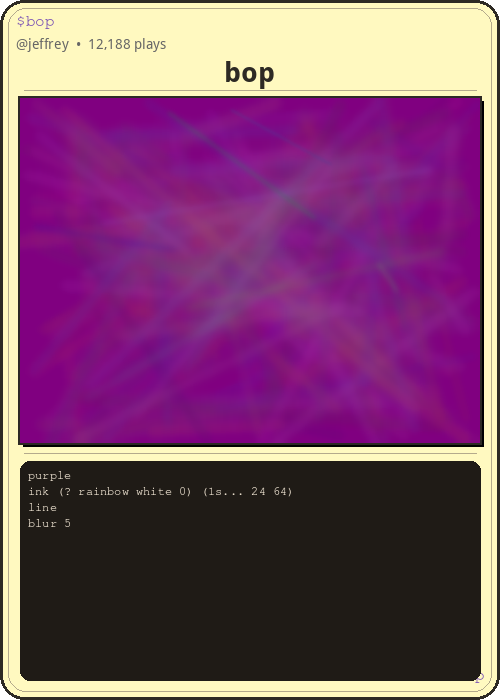
\includegraphics[height=7cm]{user-card-bop.png}%
\hfill%
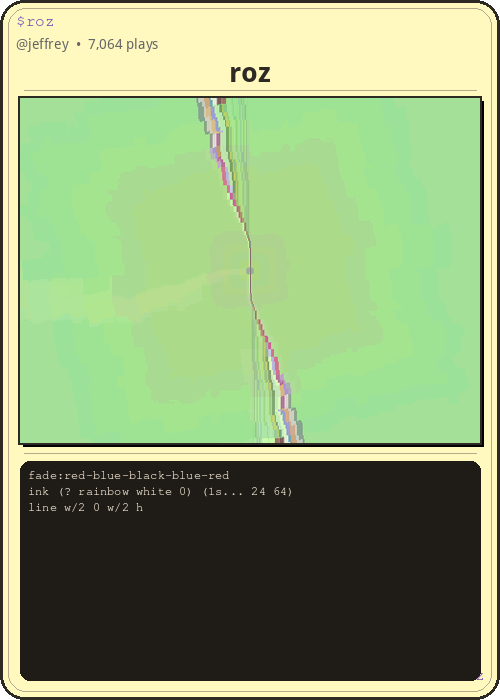
\includegraphics[height=7cm]{user-card-roz.png}%
\hfill%
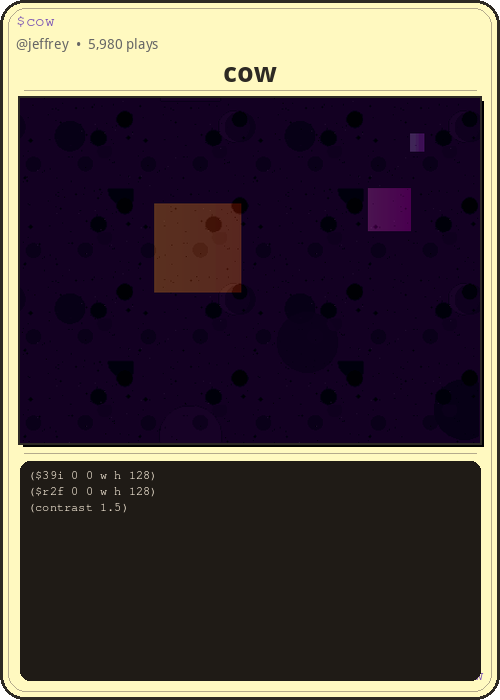
\includegraphics[height=7cm]{user-card-cow.png}%
\hfill%
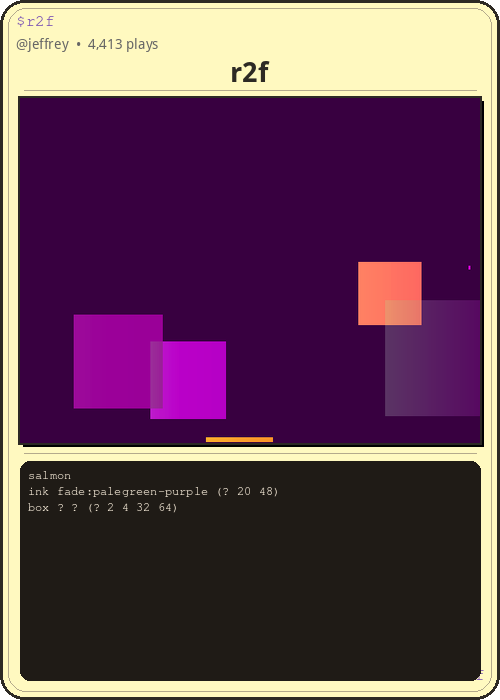
\includegraphics[height=7cm]{user-card-r2f.png}
\caption{Cuatro tarjetas del corpus vivo de \kidlisp{}, renderizadas por el servicio oven. De izquierda a derecha: \texttt{\$bop} (12.188 reproducciones---la pieza m\'as popular, 4 l\'ineas), \texttt{\$roz} (7.064 reproducciones, 3 l\'ineas), \texttt{\$cow} (5.980 reproducciones---una composici\'on que incrusta dos otras piezas v\'ia \texttt{\$39i} y \texttt{\$r2f}), \texttt{\$r2f} (4.413 reproducciones, 3 l\'ineas de colocaci\'on aleatoria de cajas). Todos por @jeffrey. Estos programas usan caracter\'isticas ausentes del int\'erprete Python---animaci\'on, aleatoriedad (\texttt{?}), gradientes (\texttt{fade:}), capas incrustadas (\texttt{\$code})---pero su c\'odigo fuente a\'un cabe en una tarjeta.}
\label{fig:user-cards}
\end{figure*}

\subsection{Qu\'e a\~naden las piezas reales}

Las tarjetas del cuaderno usan un subconjunto est\'atico de \kidlisp{}. Las piezas reales en \texttt{kidlisp.com} usan el runtime completo:

\begin{itemize}
  \item \textbf{Animaci\'on.} Los programas se re-eval\'uan cada fotograma. \texttt{frame} y \texttt{time} cambian autom\'aticamente. Una captura de un solo fotograma captura un momento de una pieza viva.
  \item \textbf{Aleatoriedad.} El operador \texttt{?} produce un valor aleatorio de una lista cada fotograma. \texttt{(ink (? red blue green))} parpadea entre colores.
  \item \textbf{Gradientes.} \texttt{fade:red-blue-black} interpola un gradiente de m\'ultiples paradas a trav\'es del lienzo, impulsado por el conteo de \texttt{frame}. Una expresi\'on reemplaza p\'aginas de matem\'aticas de color manuales.
  \item \textbf{Incrustaci\'on.} \texttt{(\$cow)} obtiene la pieza \texttt{cow} de MongoDB, la eval\'ua en un b\'ufer fuera de pantalla y compone el resultado. Las piezas se construyen sobre piezas.
  \item \textbf{Temporizaci\'on.} \texttt{1s... (zoom 0.5)} aplica un zoom cada segundo. Sin bucle de animaci\'on expl\'icito.
\end{itemize}

Estas caracter\'isticas mantienen los programas cortos mientras expanden dram\'aticamente lo que pueden expresar. \texttt{\$bop}---la pieza m\'as reproducida con 12.188 vistas---son cuatro l\'ineas: un fondo morado, tinta parpadeante arco\'iris, una l\'inea aleatoria y un desenfoque. En una tarjeta, parece un momento congelado de una pintura cin\'etica. En el navegador, lo es.

\subsection{La tarjeta como instant\'anea}

Una tarjeta de una pieza animada es necesariamente incompleta. Captura un fotograma de un proceso temporal. Esta incompletitud es parte del formato: la tarjeta te invita a teclear el c\'odigo y ver qu\'e hace realmente. La imagen est\'atica es una promesa. El c\'odigo fuente es el cumplimiento. El c\'odigo corto (\texttt{\$bop}) es el puente---tecl\'ealo en \texttt{kidlisp.com} y la tarjeta cobra vida.

% ============ 7. EN QU\'E PODR\'IAN CONVERTIRSE LAS TARJETAS ============

\section{En qu\'e podr\'ian convertirse las tarjetas}
\label{sec:futures}

El formato de tarjeta es joven. El cuaderno actual es una prueba de concepto---28 programas renderizados offline. Pero la correspondencia entre programas cortos y tarjetas f\'isicas sugiere varias direcciones.

\subsection{Tarjetas coleccionables}

Una tarjeta KidLisp es coleccionable de una manera que la mayor\'ia del software no lo es. Cada tarjeta tiene un nombre, una identidad visual, un c\'odigo corto (\texttt{\$xyz}) y un autor. Las tarjetas podr\'ian imprimirse, numerarse e intercambiarse. Las tarjetas raras podr\'ian usar caracter\'isticas oscuras del lenguaje o producir salidas inesperadamente complejas a partir de c\'odigo m\'inimo. La ``rareza'' de una tarjeta es su densidad de informaci\'on: cu\'anta complejidad visual emerge de cu\'an pocos caracteres.

\subsection{Secuencias pedag\'ogicas}

Las siete categor\'ias del cuaderno actual sugieren un orden de ense\~nanza: comenzar con cajas (coordenadas simples), pasar a l\'ineas (trigonometr\'ia), c\'irculos (radio y repetici\'on), curvas matem\'aticas (plot y seno), gr\'aficos de tortuga (movimiento relativo) y finalmente koans (expresi\'on m\'inima). Cada tarjeta ense\~na un concepto. Un profesor podr\'ia entregar a los estudiantes una baraja f\'isica y pedirles que reproduzcan cada tarjeta, la modifiquen o creen una nueva tarjeta en la misma categor\'ia.

\subsection{Partituras impresas}

En m\'usica, una partitura son instrucciones para producir un evento temporal. Una tarjeta KidLisp son instrucciones para producir un evento visual. Las tarjetas podr\'ian funcionar como partituras gr\'aficas en la tradici\'on de Cornelius Cardew, John Cage y las partituras de eventos Fluxus. Un int\'erprete recibe una tarjeta, interpreta el c\'odigo (tecle\'andolo en \texttt{kidlisp.com}, ley\'endolo en voz alta, dibuj\'andolo a mano) y produce un evento. La tarjeta es la partitura. El renderizado es una realizaci\'on posible.

\subsection{Arte postal}

A 4$\times$6 pulgadas, una tarjeta KidLisp es una postal. El frente muestra la imagen renderizada. El reverso muestra el c\'odigo fuente, el handle del autor y el c\'odigo corto para buscarlo en l\'inea. Arte postal con contenido ejecutable---el destinatario puede teclear el c\'odigo y ver la imagen regenerarse en su pantalla. La tarjeta f\'isica y el programa digital son la misma obra en dos medios.

\subsection{Papeler\'ia generativa}

Dado que el int\'erprete Python es determinista y aut\'onomo, las tarjetas pueden renderizarse por lotes para producci\'on de impresi\'on sin acceso a la red. Un conjunto de tarjetas podr\'ia imprimirse como folleto, fanzine o set en caja. El pipeline \texttt{cards-convert.mjs} ya produce tarjetas PDF de 4$\times$6 pulgadas desde el formato del art\'iculo; extender esto para incluir la salida renderizada del programa junto con el c\'odigo fuente es un pr\'oximo paso natural.

\subsection{La restricci\'on como principio generativo}

La consecuencia m\'as interesante del formato de tarjeta es c\'omo retroalimenta el lenguaje. Los programas que no caben en una tarjeta sugieren abstracciones faltantes---o sugieren que el programa hace demasiado. La restricci\'on de la tarjeta fomenta la econom\'ia: encontrar el programa de tres l\'ineas que produce la imagen m\'as interesante. Esta es una restricci\'on generativa en la tradici\'on de Oulipo---restricciones formales arbitrarias que producen resultados creativos inesperados.

% ============ 6. TRABAJO RELACIONADO ============

\section{Trabajo relacionado}

\textbf{C\'odigo impreso.} La tradici\'on de la demoscene de ``sizecoding'' (programas de menos de 256 bytes) comparte la est\'etica de programas m\'inimos que producen salida m\'axima. Las tarjetas de \kidlisp{} est\'an m\'as cerca de la tradici\'on del ``poema de c\'odigo'', donde el c\'odigo fuente mismo se lee como texto junto con su salida.

\textbf{Partituras gr\'aficas.} El \emph{Treatise} de Cardew (1967) y las \emph{Notations} de Cage (1969) establecieron que la notaci\'on visual puede servir como instrucciones de interpretaci\'on sin prescribir una realizaci\'on espec\'ifica. Las tarjetas KidLisp difieren en que son completamente ejecutables---el renderizado es determinista, no abierto a interpretaci\'on. Pero el encuadre de tarjeta-como-partitura invita a la reinterpretaci\'on: \textquestiondown qu\'e pasa si ``tocas'' la tarjeta de manera diferente cada vez?

\textbf{Juegos de tarjetas coleccionables.} Juegos como \emph{Magic: The Gathering} (1993) demostraron que las tarjetas con metadatos estructurados (nombre, tipo, texto de reglas, arte) crean ricos espacios combinatorios. Las tarjetas KidLisp tienen metadatos naturales (t\'itulo, categor\'ia, n\'umero de funciones, n\'umero de l\'ineas, complejidad de salida) que podr\'ian soportar mec\'anicas de juego similares.

\textbf{Cuadernos computacionales.} Los cuadernos Jupyter ya combinan c\'odigo y salida. El cuaderno de KidLisp Cards es un cuaderno Jupyter, pero con una restricci\'on espec\'ifica: cada celda es una tarjeta autocontenida en lugar de un paso en un c\'alculo m\'as largo. El cuaderno es una galer\'ia, no una narrativa.

% ============ 7. CONCLUSI\'ON ============

\section{Conclusi\'on}

Las tarjetas KidLisp surgen de una observaci\'on simple: cuando los programas son lo suficientemente cortos, caben en tarjetas. El formato de tarjeta---t\'itulo, imagen, fuente---convierte los programas en artefactos f\'isicos que pueden imprimirse, enviarse por correo, coleccionarse, ense\~narse y ejecutarse. El pipeline de renderizado en Python permite la producci\'on offline por lotes. El cat\'alogo de siete categor\'ias proporciona un punto de entrada curado al lenguaje.

El formato es un trabajo en progreso. La baraja actual de 28 tarjetas es un punto de partida, no una colecci\'on terminada. La pregunta no es cu\'antas tarjetas hacer sino qu\'e programas merecen ser tarjetas---qu\'e composiciones de tres l\'ineas producen im\'agenes que vale la pena sostener en la mano.

El cuaderno, el int\'erprete y el cat\'alogo de tarjetas est\'an disponibles en \url{https://github.com/whistlegraph/aesthetic-computer}. Los programas pueden crearse y compartirse en \url{https://kidlisp.com}.

\vspace{0.5em}
\noindent\textbf{ORCID:} \href{https://orcid.org/0009-0007-4460-4913}{0009-0007-4460-4913}

% ============ REFERENCIAS ============

\bibliographystyle{plainnat}
\bibliography{references}

\end{document}
